\documentclass[border=0.2cm]{standalone}

\usepackage[utf8]{inputenc}
\usepackage[T1]{fontenc}
\usepackage{amsmath}
\usepackage{helvet}
\usepackage{tikz}

\usetikzlibrary{arrows.meta}
\usetikzlibrary{positioning, calc, fit}
\usetikzlibrary{decorations.markings}
\usetikzlibrary{shapes.geometric, shapes.arrows}

\renewcommand\familydefault\sfdefault


\begin{document}

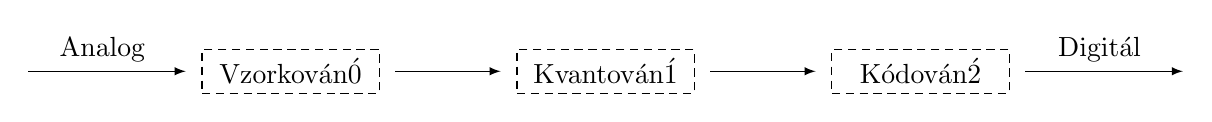
\begin{tikzpicture}[
    d arrow/.style={gray!50!black, thick, double arrow, draw, minimum width = 8pt, double arrow head extend=2pt, anchor=tip 2},
    s arrow/.style={gray!50!black,thick, single arrow, draw, minimum width = 8pt, single arrow head extend=2pt},
    block/.style={thick, draw, font=\footnotesize},
    square/.style={block, minimum size=1.5cm},
    pin/.style={font=\scriptsize}
]
    \foreach \label [count=\i from 0] in {Vzorkování, Kvantování, Kódování} {
        \draw (0, 0) ++(\i * 4, 0) node [draw, densely dashed, minimum width=2.25cm] (n\i) {$ \text{\label} $};
    }

    \draw[-latex] ($(n0.east) +(.2, 0) $) to ($(n1.west) -(.2, 0) $);
    \draw[-latex] ($(n1.east) +(.2, 0) $) to ($(n2.west) -(.2, 0) $);

    \draw[latex-] ($(n0.west) -(.2, 0) $) coordinate (a0) to ($(n0.west) -(2.2, 0) $) coordinate (a1); % node[above, align=center] {Analog};
    \draw ($ (a0)!.5!(a1) $) node[above, align=center] { \text{Analog} };

    \draw[-latex] ($(n2.east) +(.2, 0) $) coordinate (d0) to ($(n2.east) +(2.2, 0) $) coordinate (d1); % node[above, align=center] {Analog};
    \draw ($ (d0)!.5!(d1) $) node[above, align=center] { \text{Digitál} };
    
\end{tikzpicture}
\end{document}